\documentclass[border=5pt]{standalone}
\usepackage[T1]{fontenc}
\usepackage{lmodern,amsmath,amssymb,tikz}
\usetikzlibrary{arrows.meta,decorations.markings,calc,backgrounds}
\definecolor{branch}{RGB}{195,80,15}
\definecolor{branchB}{RGB}{18,125,105}
\definecolor{direct}{RGB}{37,82,156}
\definecolor{merged}{RGB}{109,57,133}
\definecolor{spoke}{RGB}{95,95,102}
\definecolor{srcgreen}{RGB}{22,120,55}
\tikzset{
  v/.style={circle,fill=black,inner sep=1.55pt},
  ins/.style={rectangle,draw=black,fill=white,line width=0.65pt,minimum size=4.6pt,inner sep=0pt},
  res/.style={line width=0.78pt,postaction={decorate},decoration={
    markings,
    mark=at position 0.48 with {\draw[line width=0.72pt,fill=white] (-0.27,-0.105) rectangle (0.27,0.105);},
    mark=at position 0.82 with {\arrow{Stealth[length=1.35mm,width=1.05mm]}}
  }},
  resns/.style={line width=0.78pt,postaction={decorate},decoration={
    markings,
    mark=at position 0.50 with {\draw[line width=0.72pt,fill=white] (-0.25,-0.10) rectangle (0.25,0.10);}
  }},
  source/.style={-{Stealth[length=1.55mm,width=1.15mm]},line width=0.75pt},
  reduce/.style={-{Stealth[length=2.0mm,width=1.45mm]},line width=0.9pt},
  lbl/.style={fill=white,inner sep=1.1pt}
}

\begin{document}
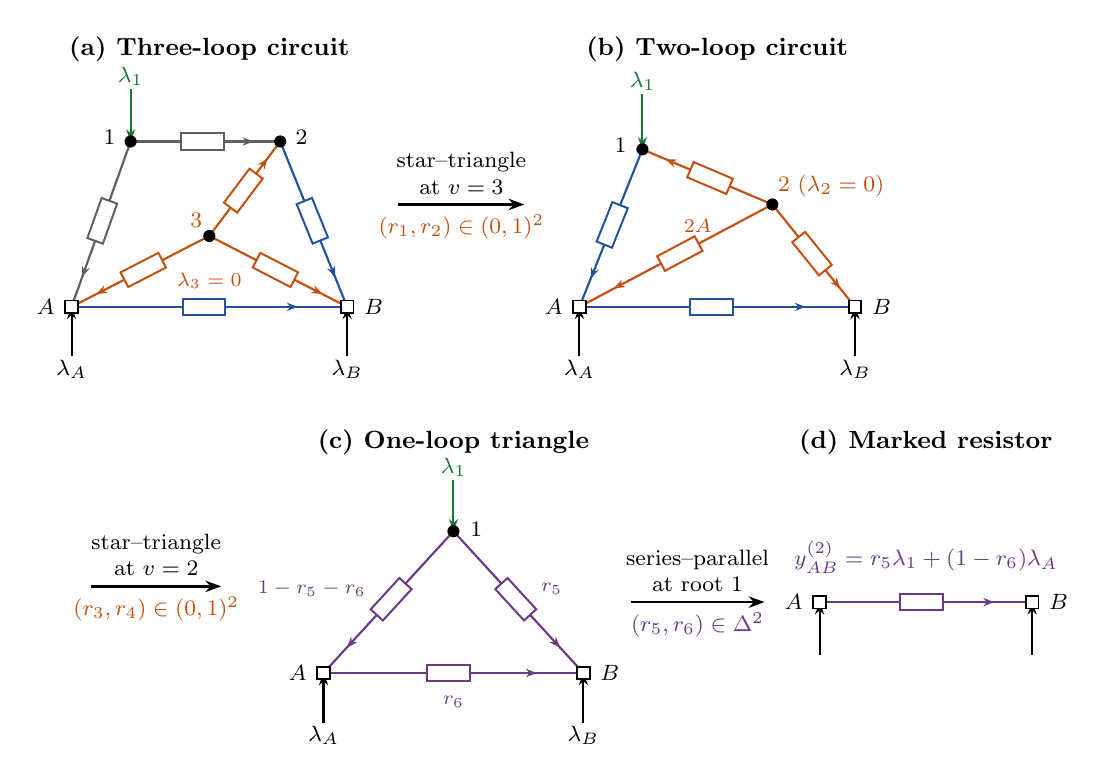
\begin{tikzpicture}[x=1cm,y=1cm,font=\footnotesize]

% Stage (a): Three-loop circuit
\begin{scope}[xshift=0cm]
  \node[font=\small\bfseries] at (1.85,3.62) {(a) Three-loop circuit};
  \coordinate (A) at (0.1,0.35);
  \coordinate (B) at (3.6,0.35);
  \coordinate (v1) at (0.85,2.45);
  \coordinate (v2) at (2.75,2.45);
  \coordinate (v3) at (1.85,1.25);

  \draw[res,spoke] (v1)--(v2);
  \draw[res,spoke] (v1)--(A);
  \draw[res,direct] (v2)--(B);
  \draw[res,direct] (A)--(B);
  \draw[res,branch] (v3)--(v2);
  \draw[res,branch] (v3)--(A);
  \draw[res,branch] (v3)--(B);

  \draw[source,srcgreen] (0.85,3.12)--(v1);
  \node[srcgreen,above,inner sep=1pt] at (0.85,3.12) {$\lambda_1$};
  \draw[source] (0.1,-0.28)--(A); \node[below,inner sep=1pt] at (0.1,-0.28) {$\lambda_A$};
  \draw[source] (3.6,-0.28)--(B); \node[below,inner sep=1pt] at (3.6,-0.28) {$\lambda_B$};

  \node[left] at (0.78,2.50) {$1$};
  \node[right] at (2.82,2.50) {$2$};
  \node[branch,above left,inner sep=1pt] at (1.80,1.32) {$3$};
  \node[branch,font=\scriptsize] at (1.85,0.68) {$\lambda_3=0$};

  \node[ins,label=left:$A$] at (A) {};
  \node[ins,label=right:$B$] at (B) {};
  \foreach \p in {v1,v2,v3}{\node[v] at (\p) {};}
\end{scope}

\draw[reduce] (4.25,1.65)--node[above,align=center]{star--triangle\\at $v=3$} node[below,branch,align=center]{$(r_1,r_2)\in(0,1)^2$} (5.85,1.65);

% Stage (b): Two-loop circuit
\begin{scope}[xshift=6.45cm]
  \node[font=\small\bfseries] at (1.85,3.62) {(b) Two-loop circuit};
  \coordinate (A) at (0.1,0.35);
  \coordinate (B) at (3.6,0.35);
  \coordinate (v1) at (0.90,2.35);
  \coordinate (v2) at (2.55,1.65);

  \draw[res,direct] (v1)--(A);
  \draw[res,direct] (A)--(B);
  \draw[res,branch] (v2)--(v1);
  \draw[res,branch] (v2)--(A);
  \draw[res,branch] (v2)--(B);

  \draw[source,srcgreen] (0.90,3.05)--(v1);
  \node[srcgreen,above,inner sep=1pt] at (0.90,3.05) {$\lambda_1$};
  \draw[source] (0.1,-0.28)--(A); \node[below,inner sep=1pt] at (0.1,-0.28) {$\lambda_A$};
  \draw[source] (3.6,-0.28)--(B); \node[below,inner sep=1pt] at (3.6,-0.28) {$\lambda_B$};

  \node[left] at (0.82,2.40) {$1$};
  \node[branch,above right,inner sep=1pt] at (2.58,1.70) {$2$ ($\lambda_2=0$)};
  \node[branch,font=\scriptsize,above left,inner sep=1pt] at (1.82,1.25) {$2A$};

  \node[ins,label=left:$A$] at (A) {};
  \node[ins,label=right:$B$] at (B) {};
  \foreach \p in {v1,v2}{\node[v] at (\p) {};}
\end{scope}

% Second row: (c) and (d)
\begin{scope}[yshift=-4.65cm,xshift=0.35cm]
  \draw[reduce] (0.0,1.45)--node[above,align=center]{star--triangle\\at $v=2$} node[below,branch,align=center]{$(r_3,r_4)\in(0,1)^2$} (1.65,1.45);

  \begin{scope}[xshift=2.85cm]
    \node[font=\small\bfseries] at (1.75,3.28) {(c) One-loop triangle};
    \coordinate (A) at (0.1,0.35);
    \coordinate (B) at (3.4,0.35);
    \coordinate (v1) at (1.75,2.15);

    \draw[res,merged] (v1)--(A);
    \draw[res,merged] (v1)--(B);
    \draw[res,merged] (A)--(B);

    \draw[source,srcgreen] (1.75,2.80)--(v1);
    \node[srcgreen,above,inner sep=1pt] at (1.75,2.80) {$\lambda_1$};
    \draw[source] (0.1,-0.28)--(A); \node[below,inner sep=1pt] at (0.1,-0.28) {$\lambda_A$};
    \draw[source] (3.4,-0.28)--(B); \node[below,inner sep=1pt] at (3.4,-0.28) {$\lambda_B$};

    \node[right] at (1.84,2.18) {$1$};
    \node[merged,left,font=\scriptsize] at (0.76,1.42) {$1-r_5-r_6$};
    \node[merged,right,font=\scriptsize] at (2.74,1.42) {$r_5$};
    \node[merged,below,font=\scriptsize] at (1.75,0.18) {$r_6$};

    \node[ins,label=left:$A$] at (A) {};
    \node[ins,label=right:$B$] at (B) {};
    \node[v] at (v1) {};
  \end{scope}

  \draw[reduce] (6.85,1.25)--node[above,align=center]{series--parallel\\at root $1$} node[below,merged,align=center]{$(r_5,r_6)\in\Delta^2$} (8.55,1.25);

  \begin{scope}[xshift=9.15cm]
    \node[font=\small\bfseries] at (1.45,3.28) {(d) Marked resistor};
    \coordinate (A) at (0.1,1.25);
    \coordinate (B) at (2.8,1.25);
    \draw[res,merged] (A)--(B);
    \draw[source] (0.1,0.58)--(A);
    \draw[source] (2.8,0.58)--(B);
    \node[merged,above=2.4mm] at (1.45,1.25) {$y_{AB}^{(2)}=r_5\lambda_1+(1-r_6)\lambda_A$};
    \node[ins,label=left:$A$] at (A) {};
    \node[ins,label=right:$B$] at (B) {};
  \end{scope}
\end{scope}

\end{tikzpicture}
\end{document}
